%%%%%%%%%%%%%%%%%%%%%%%%%%%%%%%%%%%%%%%%%%%%%%%%%%%%%%%%%%%%%%%%%%%%%%
%%%%%%%%%%%%%% Pacotes básicos obrigatório        %%%%%%%%%%%%%%%%%%%%
%%%%%%%%%%%%%%%%%%%%%%%%%%%%%%%%%%%%%%%%%%%%%%%%%%%%%%%%%%%%%%%%%%%%%%

\documentclass[12pt]{article} 
\usepackage[utf8x]{inputenc}
\usepackage[brazilian]{babel}
\usepackage{fontenc}
\usepackage{graphicx} 
\usepackage{xcolor}


%%%%%%%%%%%%%%%%%%%%%%%%%%%%%%%%%%%%%%%%%%%%%%%%%%%%%%%%%%%%%%%%%%%%%%
%%%%%%%%%%%%%% Alguns Pacotes que podemos utilizar%%%%%%%%%%%%%%%%%%%%
%%%%%%%%%%%%%%%%%%%%%%%%%%%%%%%%%%%%%%%%%%%%%%%%%%%%%%%%%%%%%%%%%%%%%%

\usepackage{indentfirst} %identa o primeiro paragrafo da seção
%\usepackage{pdflscape} % se quiser colocar uma figura na pagina deitada

%se quiser alterar as bordas da página
% \usepackage[bottom=3cm,top=3cm,left=3cm,right=3cm]{geometry} 
\usepackage[pdftex]{hyperref} %permitir \url clicável nos links
% \usepackage{subfig}

%%%%%%% Para colocar a logo da ufc na primeira página %%%%%%%%%%%%%%%%
\usepackage{wallpaper} 
\usepackage[absolute]{textpos}

%%%%%%%%%%%%%%%%%%%%%%%%%%%%%%%%%%%%%%%%%%%%%%%%%%%%%%%%%%%%%%%%%%%%%%
%%%%%%%%%%%%%% Configurando pacote para bordas  %%%%%%%%%%%%%%%%%%%%%%
%%%%%%%%%%%%%%%%%%%%%%%%%%%%%%%%%%%%%%%%%%%%%%%%%%%%%%%%%%%%%%%%%%%%%%
\usepackage[framemethod=TikZ]{mdframed} % para os frames
\mdfsetup{%
	%middlelinecolor=red,
	middlelinewidth=2pt,
	%backgroundcolor=red!20,
	roundcorner=10pt
}

%%%%%%%%%%%%%%%%%%%%%%%%%%%%%%%%%%%%%%%%%%%%%%%%%%%%%%%%%%%%%%%%%%%%%%
%%%%%%%%%%%%%% Configurando pacote para cabeçalho %%%%%%%%%%%%%%%%%%%%
%%%%%%%%%%%%%%%%%%%%%%%%%%%%%%%%%%%%%%%%%%%%%%%%%%%%%%%%%%%%%%%%%%%%%%
\usepackage{fancyhdr}
\pagestyle{fancy}
\fancyhf{}
\lhead{Fundamentos de Programação}
\rhead{UFC - Quixadá}
\fancyfoot[R]{\thepage}
\rfoot{Page \thepage}


%%%%%%%%%%%%%%%%%%%%%%%%%%%%%%%%%%%%%%%%%%%%%%%%%%%%%%%%%%%%%%%%%%%%%%
%%%%%%%%%%%%%% Configurando pacote para códigos   %%%%%%%%%%%%%%%%%%%%
%%%%%%%%%%%%%%%%%%%%%%%%%%%%%%%%%%%%%%%%%%%%%%%%%%%%%%%%%%%%%%%%%%%%%%
\usepackage{listings}
\lstset{
	language=java,
	%    language=c++,
	keywordstyle=\bfseries\ttfamily\color[rgb]{0,0,1},
	identifierstyle=\ttfamily,
	commentstyle=\color[rgb]{0.133,0.545,0.133},
	stringstyle=\ttfamily\color[rgb]{0.627,0.126,0.941},
	showstringspaces=false,
	basicstyle=\small,
	tabsize=2,
	breaklines=true,
	frame=single
}


%%%%%%%%%%%%%%%%%%%%%%%%%%%%%%%%%%%%%%%%%%%%%%%%%%%%%%%%%%%%%%%%%%%%%%
%%%%%%%%%%%%%% Definindo Atalhos %%%%%%%%%%%%%%%%%%%%%%%%%%%%%%%%%%%%%
%%%%%%%%%%%%%%%%%%%%%%%%%%%%%%%%%%%%%%%%%%%%%%%%%%%%%%%%%%%%%%%%%%%%%%


\newcommand{\code}[1]{\lstinline|#1|} %% para codigos inline
\newcommand{\ita}[1]{\textit{#1}}  %% para italico
\newcommand{\bold}[1]{\textbf{#1}} %% para negrito
\newcommand{\note}[1]{\footnote{#1}} %% para anotações laterais
\newcommand{\caps}[1]{\textbf{#1}} %% para CAPS

%%%%%%%%%%%%%%%%%%%%%%%%%%%%%%%%%%%%%%%%%%%%%%%%%%%%%%%%%%%%%%%%%%%%%%
%%%%%%%%%%% Escolha da fonte     %%%%%%%%%%%%%%%%%%%%%%%%%%%%%%%%%%%%%
%%%%%%%%%%%%%%%%%%%%%%%%%%%%%%%%%%%%%%%%%%%%%%%%%%%%%%%%%%%%%%%%%%%%%%
% Deixe as duas comentadas para usar o default Helvetica e Palatino
%\usepackage{lmodern}
%\usepackage{txfonts}



\begin{document}

\ThisULCornerWallPaper{1}{./imagens/header}
\begin{textblock}{15}(0.4, 0.4)
\noindent
\begin{center}
\LARGE{\bf{QXCode - Quixadá Coding Team}}\\
\large{\bf{Fundamentos de Programação}} \\
\large{\bf{\today}}
\end{center}
\end{textblock}

\title{\bf{Blackjack \\ Um Jogo de Cartas Inocente}}

\author{
David Sena Oliveira\thanks{sena.ufc@gmail.com}
}

\date{}

\maketitle
\thispagestyle{empty}

%#################################################################
%#################################################################
%#################################################################
%#################################################################
\section{Introdução}

\caps{O objetivo} dessa atividade é simular o jogo de Blackjack 21 entre um usuário e a mesa. Iremos implementar o baralho, a aleatoriedade, as regras do jogo, a inteligência da mesa e processar as escolhas do usuário. As opções do jogador são simplificadas em relação ao jogo original. \note{Mas ninguém impede se você quiser implementar o jogo completo, OK?!}. 

Imagino que você vai implementar em C, C++ ou Python. Vamos dar algumas dicas para essas linguagens.

Nosso baralho terá as seguintes cartas: 
\ita{[A, 2, 3, 4, 5, 6, 7, 8, 9, 10, J, Q, K]}. 
Nos referiremos às cartas pela sua letra. Pra não confundir, vamos utilizar sempre o itálico.


%A sequencia da figura \ref{fig:blackjack} ganha o jogo.

\begin{figure}[h]
\centering
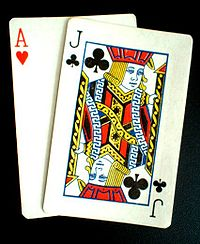
\includegraphics[width=0.3\linewidth]{./imagens/blackjack}
%\label{fig:blackjack}
\end{figure}

\section{Links úteis}
Os seguintes links podem lhe ajudar a conhecer melhor as regras do jogo:

\url{pt.blackjack.org/regras/} 

Você também pode jogar online uma simulação bem parecida com a que vamos implementar para compreender as regras.

\url{http://jogosonline.uol.com.br/blackjack-gentleman-s-bet_43651.html}
\section{Como funciona}

\begin{figure}[h]
	\centering
	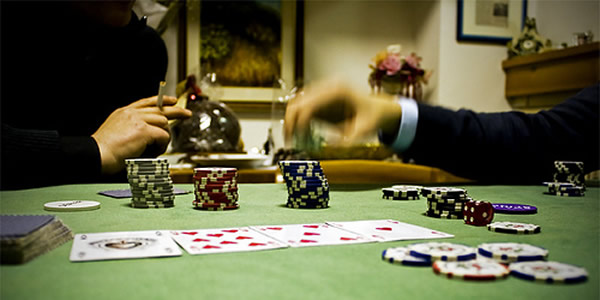
\includegraphics{imagens/mesa}
\end{figure}


\caps{O resumo:} O dealer\note{O funcionário que coordena a mesa} pede uma carta para mesa e duas para o jogador deixando todas viradas para cima. O jogador vai pedindo cartas à mesa. Seu objetivo é chegar o mais perto que puder de ter uma mão com valor 21. Se ele passar de 21 ele automaticamente perde. Se ele fizer exatos 21 pontos ele ganha. 

Após o jogador parar sua jogada, supondo que ele não estourou o limite, a mesa(máquina) vai puxar as cartas para tentar vencer o jogador. A mesa tem a vantagem do empate. Se ela fizer a mesma pontuação do jogador ela ganha. Se ela estourar ela perde. \note{No nosso modelo, a mesa ou ganha ou estoura, porque ela não vai se contentar em perder.}

\caps{O valor das cartas:} As cartas \ita{2, 3, 4, 5, 6, 7 ,8, 9, 10} têm um valor igual a seu número. Os naipes não influenciam o valor das cartas.
\note{O quatro de paus possui o mesmo valor que o quatro de ouros, por exemplo.} 
Se um jogador receber as seguintes cartas: \ita{[2, 5 e 8]}, o valor de sua mão equivale a soma das 3 cartas, resultando em 15. 

As cartas \ita{J, Q, K} são todas equivalentes ao valor 10. Se um jogador possui a mão \ita{2, 8, Q}, o valor total de sua mão é 20. 
\note{20 é a segunda pontuação mais a segunda pontuação mais alta do jogo, perdendo apenas do 21.}

\caps{A última carta}, o \ita{A}, tem um valor especial no jogo de Blackjack. O \ita{A} pode valer \bold{1} ou \bold{11}, dependendo do que que for mais vantajoso para o jogador. A regra é: pense no \ita{A} como valendo \bold{11}, se isso fizer o jogador estourar, faça o \ita{A} valer 1.

\section{Implementação}
\caps{Nós iremos implementar} o modelo com um jogador e a mesa. O jogador possui apenas duas opções: Pedir Carta (Hit) ou Parar. O fluxo do jogo é o seguinte:


\itemize{
	\item O jogador inicia com 2 cartas e a mesa com 1 carta.
	
	\item O jogador pode pedir quantas cartas quiser até parar
	ou estourar o valor de 21.
	
	\item Se o jogador parar sem estourar, a mesa vai jogar até
	vencer o jogador ou estourar. Se a mesa tiver a mesma
	quantidade de pontos do jogador ela vence.
}

Nos trechos que representam a saída do terminal, os símbolos \code|>>| representam que o programa para e espera a entrada do usuário.

\begin{mdframed}[nobreak=true]
	\centering{Exemplo: Jogador perdendo.}
	
	\begin{verbatim}
	Iniciando Rodada:
	# Mesa recebe  7 - Total  7 [ 7 ]
	# Voce recebe  A - Total 11 [ A ]
	# Voce recebe  2 - Total 13 [ A 2 ]
	Pedir = 1, Parar = 2 
	>> 1
	
	# Voce recebe  3 - Total 16 [ A 2 3 ]
	Pedir = 1, Parar = 2 
	>> 2
	
	# Mesa recebe  2 - Total  9 [ 7 2 ]
	# Mesa recebe  7 - Total 16 [ 7 2 7 ]
	# Mesa (16), Voce (16)
	Voce perdeu!
	\end{verbatim}
\end{mdframed}

\note{Essa saída de terminal mostra um modelo de interação com o usuário. Desde que respeitadas as regras, você pode dar 
	a cara que quiser pro seu programa. Aqui, rodamos o programa duas vezes, uma exemplificando o jogador ganhando e outra com ele perdendo.}

\begin{mdframed}[nobreak=true]
	\centering{Exemplo: Jogador ganhando.}
	\begin{verbatim}
	Iniciando Rodada:
	# Mesa recebe  7 - Total  7 [ 7 ]
	# Voce recebe  A - Total 11 [ A ]
	# Voce recebe  2 - Total 13 [ A 2 ]
	Pedir = 1, Parar = 2 
	>> 1
	
	# Voce recebe  Q - Total 13 [ A 2 Q ]
	Pedir = 1, Parar = 2 
	>> 1
	
	# Voce recebe  5 - Total 18 [ A 2 Q 5 ]
	Pedir = 1, Parar = 2 
	>> 2
	
	# Mesa recebe  8 - Total 15 [ 7 8 ]
	# Mesa recebe  7 - Total 22 [ 7 8 7 ]
	
	# Mesa (22), Voce (18)
	Voce Ganhou
	\end{verbatim}
\end{mdframed}


\section{Melhorias}

Deixo aqui algumas sugestões pra sua diversão.
\begin{enumerate}
	\item Implementar um laço no qual o jogador continua jogando até que decida parar.
	\item Implementar um esquema de apostas no qual o jogador decide quanto quer apostar antes da rodada. O jogador pode começar com uma quantia fixa de dinheiro. Se ele ganhar a rodada, o dinheiro é adicionado na conta dele. Se ele perde, então, a, um, então ele perde.
	\item Montar um ou dois baralhos com as cartas e embaralhar. Retirar então as cartas, e após a rodada, elas vão para o montante até que o baralho termine. 
	\item Implementar o jogo com mais de um jogador. Nele, a mesa vai precisar de regras um pouco diferentes. Consulte a wiki sobre Blackjack para entender mais.
\end{enumerate}

\end{document}